\chapter{Desenvolvimento do projeto}
\label{chap:metod}
 Nesta seção, serão apresentados os métodos e processos utilizados para o desenvolvimento do portfólio digital, incluindo a metodologia adotada, a arquitetura geral do sistema, os requisitos técnicos e a modelagem dos processos. O objetivo é fornecer uma visão clara e estruturada das etapas envolvidas na criação do portfólio, desde a concepção até a implementação.

\subsection{Metodologia do projeto}
    A metodologia adotada para o desenvolvimento deste portfólio digital é baseada no modelo ágil, que prioriza a flexibilidade, a colaboração e a entrega incremental de valor. O processo foi dividido em etapas, começando com o levantamento de requisitos, seguido pela modelagem do sistema, prototipagem e testes. Essa abordagem permite uma adaptação rápida às mudanças nas necessidades do cliente e garante que o produto final atenda às expectativas.

\section{Ideação}
%escrever oq sera apresentado

A fase de ideação foi crucial para o desenvolvimento do portfólio digital, onde foram levantadas as necessidades e expectativas do cliente. A equipe realizou reuniões com o cliente para entender suas demandas, preferências estéticas e funcionais, além de analisar portfólios digitais similares no mercado. Essa etapa inicial permitiu a definição clara dos objetivos do projeto e a identificação dos requisitos essenciais.

\subsection{Arquitetura Geral}
 A estrutura da arquitetura do portfólio digital foi concebida para ser intuitiva e responsiva, garantindo uma experiência de usuário fluida em diferentes dispositivos. A camada de apresentação é responsável pela interface do usuário. Dando a ela um design responsivo, utilizando HTML e CSS para a estrutura e estilo, respectivamente. O JavaScript foi integrado para adicionar interatividade e dinamismo à interface como algumas animações.

 \begin{figure} [h!]	
    \centering

    \caption{Arquitetura Geral}
    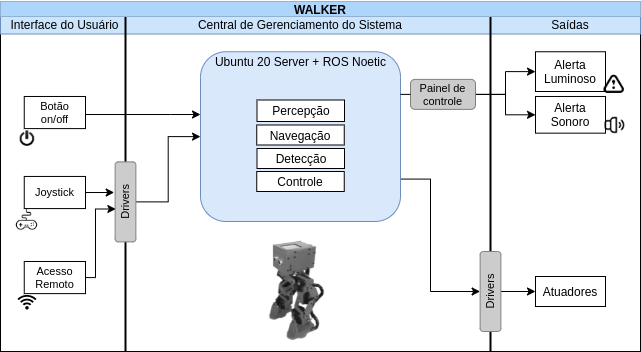
\includegraphics[width=0.8\textwidth]{general_architecture}
    \caption*{Fonte: Autoria própria.}
    \label{fig:Arquitetura geral}
\end{figure}	

Para a central de gerenciamento do sistema utilizou-se o sistema operacional \textit{Ubuntu} 20.04 junto ao framework de robótica ROS \textit{Noetic}. Neste cojunto se encontram as principais funcionalidades do robô: percepção, navegação, detecção e controle. Por fim, no conjunto de saídas estão os atuadores e os alertas sonoro e luminoso.

\subsection{Requisitos técnicos}

%desdobramento da função qualidade
% \subsection{Quality Function Deployment}
% \textit{Quality Function Deployment} é uma ferramenta de qualidade que auxilia na conversão das demandas do cliente em características de qualidade do produto. Dessa forma, no primeiro ciclo do QFD foram analisados os requisistos do cliente e os requisitos técnicos necessários, sinalizando os pontos mais importantes e as relações entre estes. O resultado foi exposto na \ref{fig:QFD}

% \begin{figure} [h!]	
%     \centering
%     \caption{ Primeiro ciclo QFD}
%     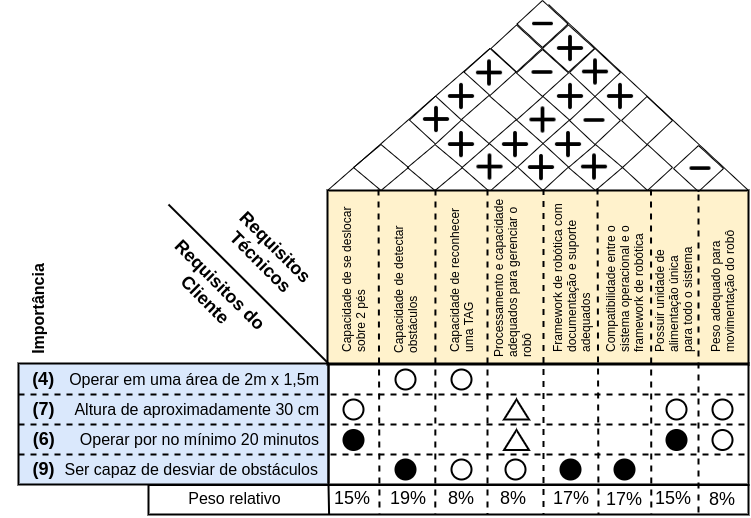
\includegraphics[width=0.8\textwidth]{Figures/QFD}
%     \caption*{Fonte: Autoria própria.}
%     \label{fig:QFD}
% \end{figure}
%  Através do QFD foi possível observar 

% % %--------- NEW SECTION ----------------------
% % \section{Interface do Usuário}
% % \label{sec:ui}
% % \lipsum[1]

% % %--------- NEW SECTION ----------------------
% % \section{Simulação do sistema}
% % \label{sec:sim}
% % \lipsum[2-4]
\subsection{Modelagem dos processos}
